\documentclass{standalone}
\usepackage{tikz}
%\usepackage{latexmk}
\usetikzlibrary{automata, arrows}

\begin{document}
	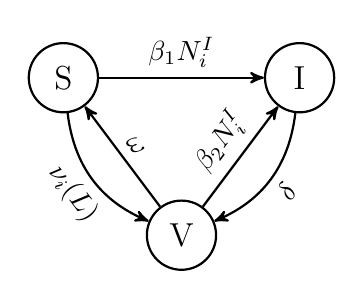
\begin{tikzpicture}[->, >=stealth', auto, thick, node distance=3cm]
		\tikzstyle{every state}=[fill=white,draw=black,thick,text=black,scale=1,font=\large]
		
		\node[state] at (0, 0)  (S)  {S};
		\node[state] at (3, 0)  (I)  {I};
		\node[state] at (1.5, -2) (V)  {V};
		
		\path
		(S) edge[sloped] node[above]{$\beta_1 N^I_i$} (I)
		(V) edge[sloped] node[above]{$\omega$} (S)
		(S) edge[sloped, bend right=30] node[below]{$\nu_i(L)$} (V)
        (I) edge[sloped, bend left=30] node[below]{$\delta$} (V)
		(V) edge[sloped] node[above]{$\beta_2 N^I_i$} (I);
	\end{tikzpicture}
\end{document}
